\chapter{Transaktionssysteme}
Die Verarbeitung von Informationen in einem Rechnernetzwerk stellt je nach Anwendungsfall verschiedenste Ansprüche an das verarbeitende System. Eine Transaktion selbst ist nach \cite{rahm1993HochleistungsTransaktionssysteme} eine Gruppe von zusammengehörenden Operationen welche gemeinsam das \textit{ACID} Prinzip, siehe Abschnitt \ref{sec:transactionTheory:acid}, einhalten und somit keine Datenanomalien oder Inkonsistenzen zulassen. \\
Durch den rapiden Anstieg an Anfragen an ein Transaktionssystem sowie die dadurch erfolgte Verteilung der Systeme, wie in \cite{li2017research} beschrieben, haben sich die Ansprüche an Transaktionssysteme in den letzten Jahren verändert. Die Verteilung von Datenverarbeitenden und Persistierenden Systemen führt zu neuen Herausforderungen und andere Kriterien, nicht zuletzt wegen dem \textit{CAP-Theorem}, siehe Kapitel \ref{sec:distributedSystems:capTheorem}, welche in diesem Kapitel diskutiert werden. 

SAMUEL

\section{Transaktionskonzepte}
Ein Transaktionssystem muss nach \cite{rahm1993HochleistungsTransaktionssysteme}, einem definierten Konzept folgen und dieses jederzeit garantieren können, um so Transaktionen zu verarbeiten. Dabei haben sich zwei Grundlegende Konzepte, \textit{ACID} und \textit{BASE}, entwickelt, auf welche nachfolgend eingegangen wird. Welches der beiden Konzepte sich in der Praxis besser verwendet lässt, hängt vom Anwendungsfall ab. Weiters
unterscheidet sich das Ziel dieser zwei Konzepte laut \cite{EdlichFriedlandHampeBrauer201010} grundsätzlich, weshalb sie sich zum teils nur schwer vergleichen lassen. Demnach ist \textit{ACID} mehr auf die Garantierung der Konsistenz hin optimiert, während \textit{BASE} die Verteilung der Anwendung priorisiert.

\subsection{ACID}\label{sec:transactionTheory:acid}
Der Begriff \textit{ACID} steht für die vier Eigenschaften \textit{Atomarität}, \textit{Konsistenz}, \textit{Isolation} und \textit{Dauerhaftigkeit}. Ein \textit{ACID} basierendes System gilt als restriktives Transaktionssystem welches durch die, vor und nach einer Transaktion,  immer geltenden Bedingungen von allen vier Eigenschaften nur äußert schwer verteil-, und skalierbar ist \cite{PritchettBASE}.\\
Ein System welches \textit{ACID} erfühlt, bietet laut \cite{haerder198Acid} für eine Transaktion immer folgende vier Eigenschaften.

\begin{description}
    \item[Atomarität] Alle Operationen welche sich innerhalb einer Transaktion befinden werden atomar ausgeführt. Das Bedeutet es wird entweder alles ausgeführt oder garnichts. Um das zu ermöglichen, muss das Transaktionssystem gewährleisten können, dass bei einem Rollback der Transaktion bereits ausgeführte Operationen auch wieder zurückgesetzt werden kann. 
    \item[Konsistenz] Bei Beendigung einer Transaktion ist sichergestellt, das sich die Datenbank in einem Konsistenten zustand befindet. Auch wird eine Transaktion nur erfolgreich abgeschlossen wenn alle Integrationsbedingungen des darunterliegenden Datenschemas erfühlt sind. 
    \item[Isolation] Eine gerade in Ausführung befindliche Transaktion wird von einer anderen Transaktion nicht beeinflusst. Die Isolation der Transaktion bewirkt, dass sich jede Transaktion so verhalten kann, als wäre sie die einzige im gesamten System.
    \item[Dauerhaftigkeit] Wird eine Transaktion erfolgreich abgeschlossen, muss vom Transaktionssystem garantiert werden können, das sich die Daten der Transaktion dauerhaft im System befinden. Durch diese Eigenschaft kann sich der Ersteller der Transaktion, im Falle das diese erfolgreich Abgeschlossen wird, darauf verlassen, dass die Daten im System enthalten sind.
\end{description}
Um diese vier Eigenschaften auch in einem verteilten System zu Garantieren ist laut \cite{PritchettBASE} ein zwei Phasen Commit erforderlich. In diesem werden in einer erster Commit Phase alle Beteiligten Komponenten gefragt ob sie die änderungen durchführen können. Wird dies von allen bestätigt, beginnt die zweite Phase. Hier werden der Commit dann von allen beteiligten tatsächlich ausgeführt. Durch die Gewährleistung von Konsistenz über alle beteiligten Rechner ist demnach die Verfügbarkeit nach \textit{CAP} nicht garantiert und je nach Grad der Skalierung wird diese auch verringert.

\subsection{BASE}\label{sec:transactionTheory:base}
Ist jedoch die Verfügbarkeit in einem speziellen Anwendungsfall wichtiger als die jederzeit gültige Konsistenz wie in \textit{ACID} so muss eine anderes Transaktionskonzept verwendet werden. Das in \cite{PritchettBASE} beschriebene Konzept \textit{BASE} tauscht Verfügbarkeit durch Konsistenz indem es Konsistenz hinter der Verfügbarkeit einordnet. \\
\textit{BASE} steht für \textit{basically available, soft state, eventually consistent} und garantiert keine Konsistenz, versucht diese jedoch sie so gut wie möglich einzuhalten. Das wird durch die so genannte eventuelle Konsistenz erreicht. Demnach befindet sich ein System nicht immer in einem Konsistenten zustand, jedoch versucht es diesen Zustand mit abgleich von anderen Komponenten zu erreichen. Dadurch kann der Durchsatz einer Anwendung erhöht werden. Die Konsistenz der Daten bezieht sich jedoch bei \textit{BASE} ausschließlich auf die korrektheit der Daten und nicht, wie bei \textit{ACID}, auch auf die Integrität dieser \citep{EdlichFriedlandHampeBrauer201010}. Weiters bewirkt \textit{BASE} auch durch die Implementierung eines \textit{Soft State}, das geschriebene Daten nicht direkt auf allen beteiligten Komponenten verfügbar sind. Diese werden nach und nach auf die beteiligten Rechner gespielt was wiederum zu erhöhung der erreichbarkeit führt, da auf ein zwei Phasen Protokoll verzichtet werden kann \citep{EdlichFriedlandHampeBrauer201010}.

\section{Event Sourcing}
Bei gängigen Implementierungen verschiedenster Datenbanksystemen wird immer der aktuelle Zustand eines Tupels in der Datenbank gespeichert. Das führt dazu, dass bei Abfragen an das System der aktuelle Wert aus der Datenbank ausgelesen werden muss. Einen gänzlich anderen Ansatz wird beim \textit{Event Sourcing}, wie in \cite{vernon2013implementing} beschrieben, verwendet. Anstatt die Änderung an einem Datensatz direkt am Datensatz selbst vorzunehmen, wird beim \textit{Event Sourcing} nur das Event selbst, welches zu der Änderung führt, abgespeichert. Der Zustand des betroffenen Datensatzes selbst wird von der Datenbank nicht gehalten. Das Event selbst beschreibt was exakt vorgefallen ist. Wird so der Name einer Person verändert, wird das Event \textit{NameChanged} mit dem neuen Namen und eine Identifikation der betroffenen Person abgespeichert.Den aktuellen Zustand einer Identität wird jedoch nicht mehr von der Datenbank verwaltet, sondern von der Applikation selbst. Durch das Einspielen von allen bereits geschehenen Events, in der gleichen Reihenfolge wie sie aufgetreten sind, kann der aktuelle Zustand jederzeit wieder hergestellt werden. Weiters ergibt sich durch das Persistieren von allen Events, eine lückenlose Aufzeichnung wie der aktuelle Systemstatus zustande gekommen ist. \cite{vernon2013implementing} 
Jedoch ist das Einspielen von Events, ab einer gewiesen Anzahl an Events, Ressourcen und Zeitintensiv. In \cite{vernon2013implementing} wird deshalb empfohlen sogenannte Snapshots  anzulegen. Dabei wird immer wieder eine Zusammenfassung aller bisher Events erstellt, und diese Aggregation an Eventdaten gespeichert.  Alle Einspielungen danach können aufgrund dieses Snapshot durchgeführt werden. Wie oft diese Snapshots erstellt werden, kommt auf den Anwendungsfall an. Meist wird jedoch nach eintreten einer bestimmten Anzahl an Events ein Snapshot erstellt. \\
In einem  \textit{Event Sourcing} Systems sind aufgetretene Events unveränderbar. Sind Fehler in Events passiert oder müssen rückgängig gemacht werden, so wird ein neues Event eingefügt, welches das fehlerhafte Event wieder neutralisiert. Jedoch sind technisch diese Events vorhanden, sie werden jedoch durch neue ,inverse Events  neutralisiert \citep{vernon2013implementing}. 
\subsection{Zusammenhang mit CQRS}
Laut \cite{vernon2013implementing} werden im Kontext von \textit{Event Sourcing} Instanzen oder Tupels als Aggregat bezeichnet. Diese Aggregate horchen auf  Events, welche im gesamten System empfangen werden können, und ändern dementsprechend ihren Zustand. Da eine Event basierte Datenbank nicht dazu geignet ist Daten abzufragen, oder gar verbindungen unter den Daten (\textit{Joins}) zu bilden, wird ein anderes Konzept benötigt. In \cite{vernon2013implementing} wird dafür das \textit{Command-Query-Responsibility-Segregation}, kurz \textit{CQRS}, im zusammenhang mit \textit{Event Sourcing} empfohlen. \\
Bei \textit{CQRS} werden dabei, laut \cite{cqrsYoung2010}, Abfragen und  Befehle strikt voneinander getrennt. So kann ein Teil der Applikation sich darauf spezialisieren Befehle zu übernehmen und der andere Teil spezialisiert sich auf die möglichen Leseanfragen an das System. Im zusamenhang mit \textit{Event Sourcing} horch die Leseseite der \textit{CQRS} Komponente auf Events und kann somit seine Daten für zukünftige Lesezugriffe aktualisiert. Im gegensatz dazu werden bei Befehlen an das System nur Events an die \textit{Event Sourcing} Komponente versendet. Diese persistiert die Events und verteilt sie wieder im gesamten System. In Abbildung \ref{fig:transactionTheory:eventSourcing:cqrs} ist eine vereinfachte Abbildung einer \textit{CQRS} Architektur mit \textit{Event Sourcing} zu sehen. In der Abbildung ist zu sehen das zwei \textit{Query Handler} auf Events horchen. Tritt ein relevantes Event auf, so aktualisierten die Handler das zwischengespeicherte Resultat. Dieses kann schließlich bei Abfragen des Benutzers direkt zurückgegeben werden. Somit entfallen aufwendige Datenbankabfragen und Synchronisierungsmechanismen. \\
\begin{figure}
    \centering
    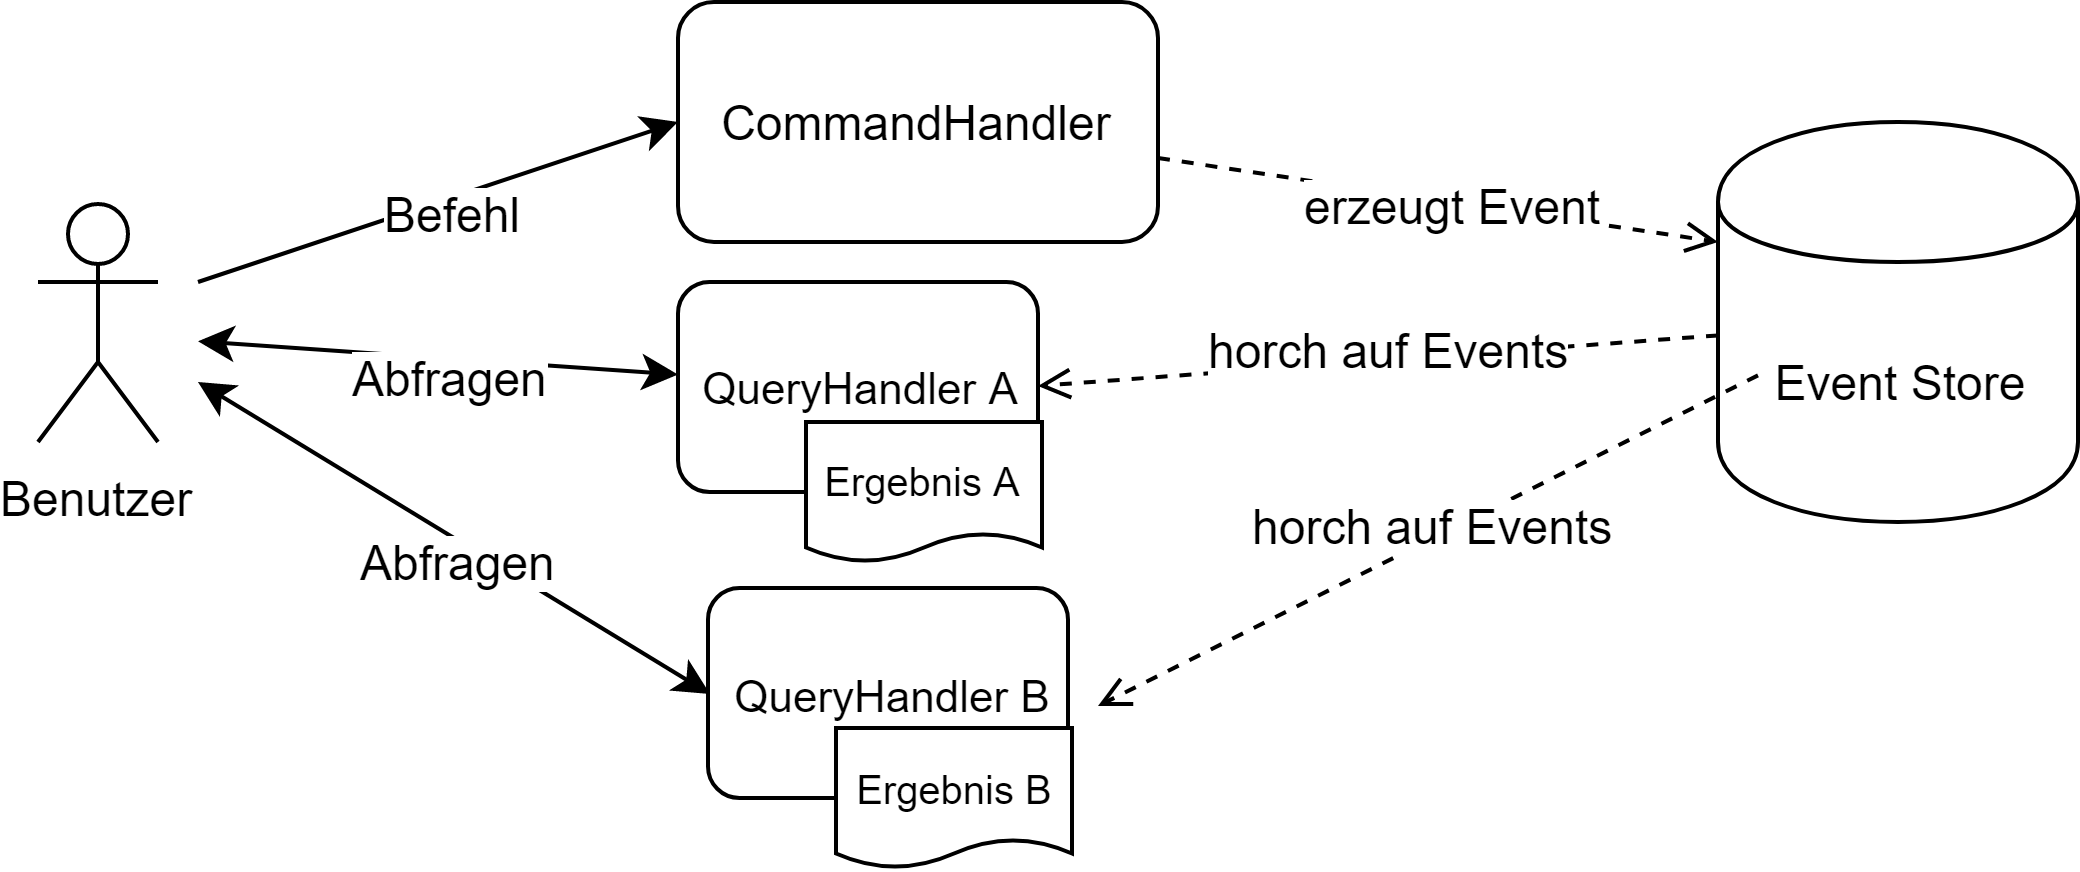
\includegraphics[width=\linewidth]{gfx/other/eventSourcingCqrs}
    \caption{Schematische, vereinfachte Darstellung von \textit{CQRS} mit \textit{Event Sourcing}.}
    \label{fig:transactionTheory:eventSourcing:cqrs}
\end{figure}
